\documentclass[11pt]{article}
\usepackage{tikz}
\usepackage{pgfplots}
\usepackage{graphicx}
\usepackage{amsmath}
\usepackage{amssymb}

\usetikzlibrary{shapes.geometric, arrows}
\tikzstyle{item} = [rectangle, rounded corners, minimum width=3cm, minimum height=1cm,text centered, draw=black, fill=red!30]\tikzstyle{arrow} = [thick,->,>=stealth]

% Margins
\topmargin=-0.45in
\evensidemargin=0in
\oddsidemargin=0in
\textwidth=6.5in
\textheight=9.0in
\headsep=0.25in

\title{SAT solvers portfolio for abstract argumentation}
\author{
    Christophe Yang \\
    Quentin Januel \\
    Sylvain Declercq
}
\date{\today}

\begin{document}

\maketitle
\newpage

\tableofcontents
\newpage

\section{Introduction}
Hello, World!

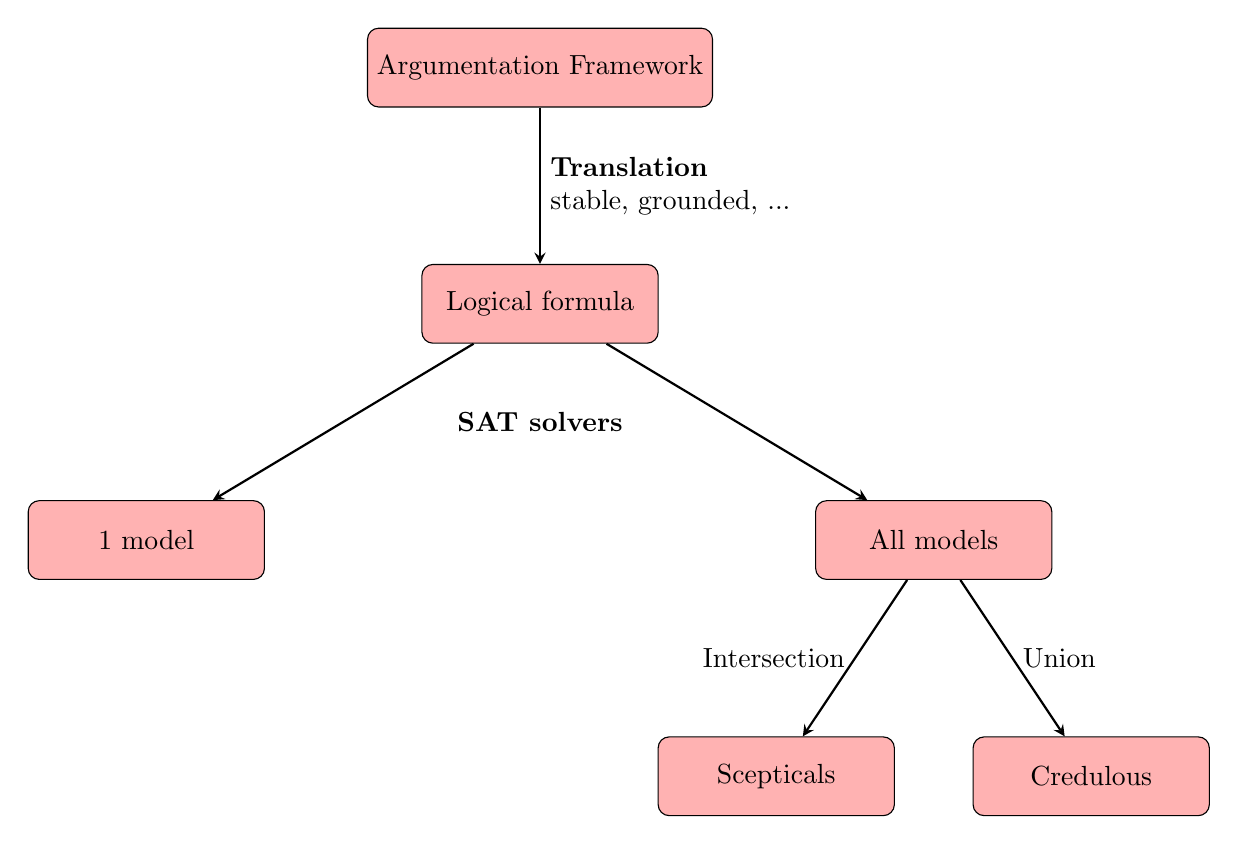
\begin{tikzpicture}[node distance=3cm]
\node(af)[item]{Argumentation Framework};
\node(log)[item, below of=af]{Logical formula};
\draw[arrow] (af) -- node[anchor=west, text width=4cm]{\textbf{Translation}\\stable, grounded, ...} (log);
\node(sat1)[item, below of=log, xshift=-5cm]{1 model};
\node(satall)[item, below of=log, xshift=5cm]{All models};
\node[below of=log, yshift=1.5cm]{\textbf{SAT solvers}};
\draw[arrow] (log) -- (sat1);
\draw[arrow] (log) -- (satall);
\node(scept)[item, below of=satall, xshift=-2cm]{Scepticals};
\node(cred)[item, below of=satall, xshift=2cm]{Credulous};
\draw[arrow] (satall) -- node[anchor=east]{Intersection} (scept);
\draw[arrow] (satall) -- node[anchor=west]{Union} (cred);

\end{tikzpicture}

\end{document}
